\Question
{باندهای عملیاتی در شبکه‌های تلفن‌همراه}
{
	باندهای عملیاتی تلفن همراه در کشورهای مختلف متفاوت است که از طریق سایت 
	\lr{spectrummonitoring} 
	\LTRfootnote{\href{https://www.spectrummonitoring.com/frequencies.php}{https://www.spectrummonitoring.com/frequencies.php}}
	قابل مشاهده است. در 
	\autoref{fig:iran-mobile}
	باندهای عملیاتی ایران که به اپراتورهای مختلف اختصاص داده‌ شده، قابل مشاهده است.

\begin{figure}[H]
    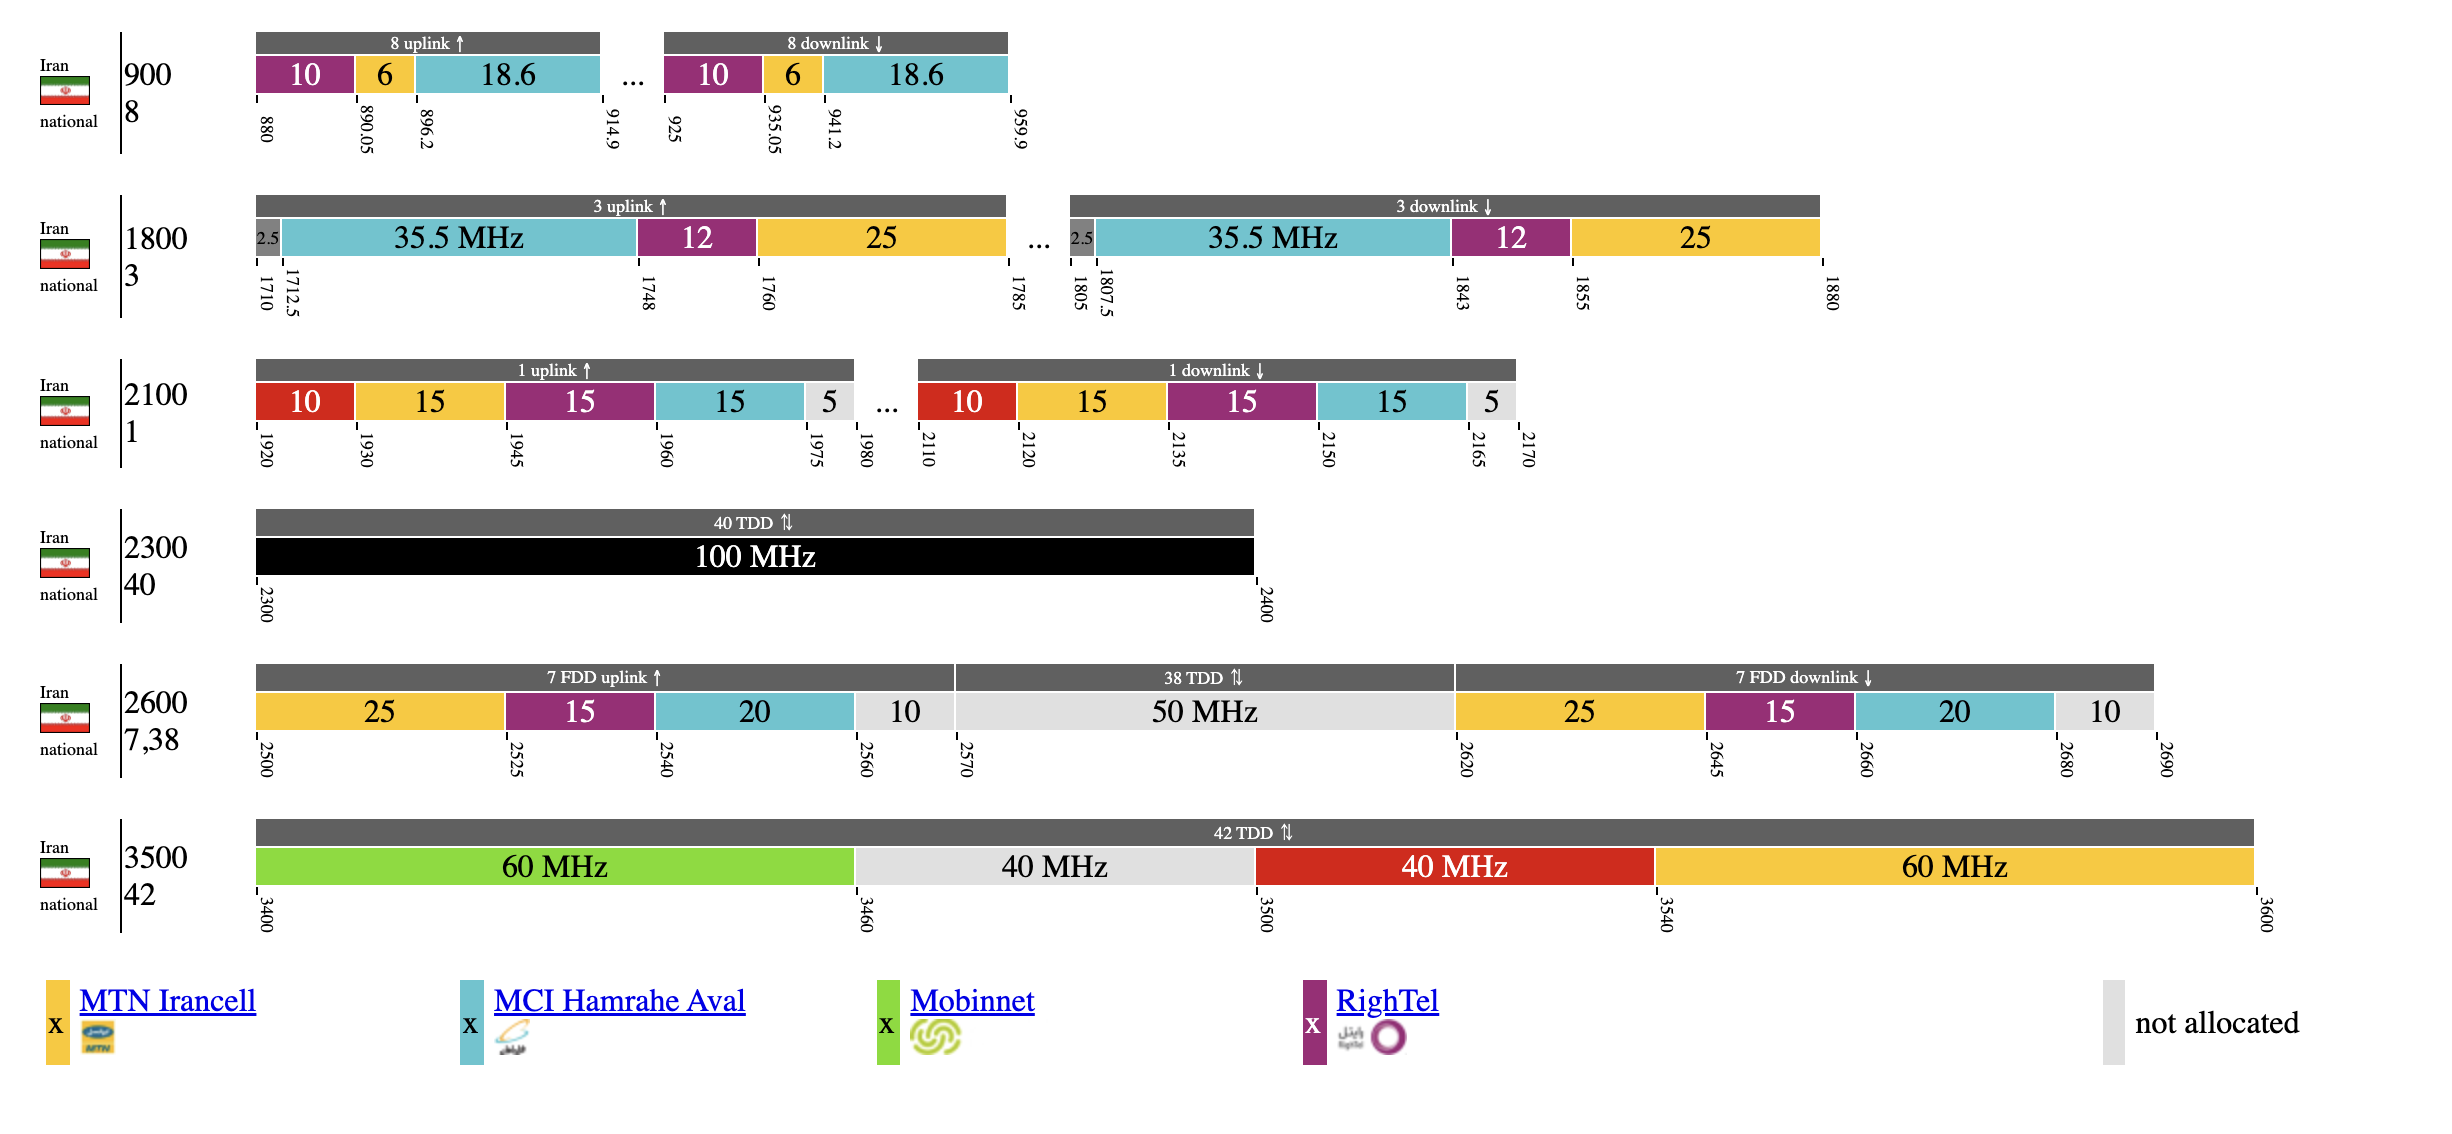
\includegraphics[width=1\columnwidth]{Images/Mobile-Frequencies-Iran.png}
    \centering
    \caption{باندهای شبکه‌های تلفن همراه در ایران}
    \label{fig:iran-mobile}
\end{figure}

باندهای نسل‌های مختلف از نظر فرکانسی هم قابل بررسی اند. به عنوان مثال در جدول‌های موجود در این 
\LTRfootnote{\href{https://en.wikipedia.org/wiki/LTE_frequency_bands}{LTE frequency bands
}}
پیوند، باندهای فرکانسی مربوط به نسل ۴ شبکه‌های تلفن همراه نمایش داده شده‌اند.
}